\section{Corrosion Resistance of Austenitic Stainless Steels}



\subsection{Passive Film Protection of Chromium}

The addition of Chromium improves the resistance of stainless steel to corrosion by orders of magnitude.  A very thin passive oxide layer, 20-30 angstroms in width, forms when the surface is exposed to an environment containing oxygen.  The protective layer is self repairing an, if the surface is damaged, the oxide layer reforms in the presence of oxygen.

When the steel is in an environment containing oxygen, electrons in the metal tunnel through the surface.  As an oxidizing agent, the nearby oxygen atoms readily accept the electrons.  A strong electric field forms between positive ions within in the metal and the negatively charged oxygen atoms \cite{medicalmetals133}.  

Iron at the surface of the forming oxide layer is preferrentially dissolved away over chromium \cite{kirchheimcc} and chromium ions within the oxide layer have a lower mobility than iron ions \cite{kirchheimpassive}.  Nickel remains in place within the alloy, and this leads to an enrichment of Chromium oxide in the passive layer.  Once the layer is thick enough to reduce the electric field across it, the formation of the layer stops.  As mentioned previously, this is at a layer thickness of 2-3nm for stainless steel.




\subsection{Sensitization and Passive Film Removal}




\begin{figure}[tbp]
  \begin{center}
    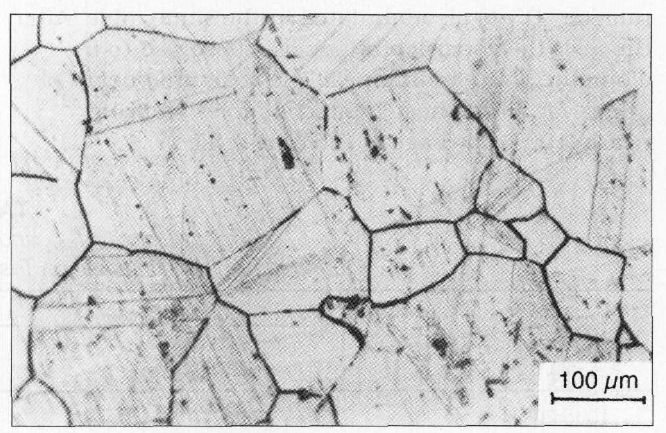
\includegraphics[width=7.0cm]{chapters/background_austenitic_steels_in_nuclear/images/grainboundaries.png}
    \caption{Graph caption}
    \label{image:flux1}
  \end{center}
\end{figure}



\subsection{Addition of Molybdenum}

A common austenitic stainless steel is 304 and this relies heavily on the passive film due to a high content of Chromium, ranging from 17.5% to 20% for grades 304, 304L and 304H.  A similar Stainless Steel, 316, has slighly less Chromium, slightly more Nickel and 2-3% Molybdenum, an element not present in 304 stainless steel.

Molybdenum 



\begin{figure}[tbp]
  \begin{center}
    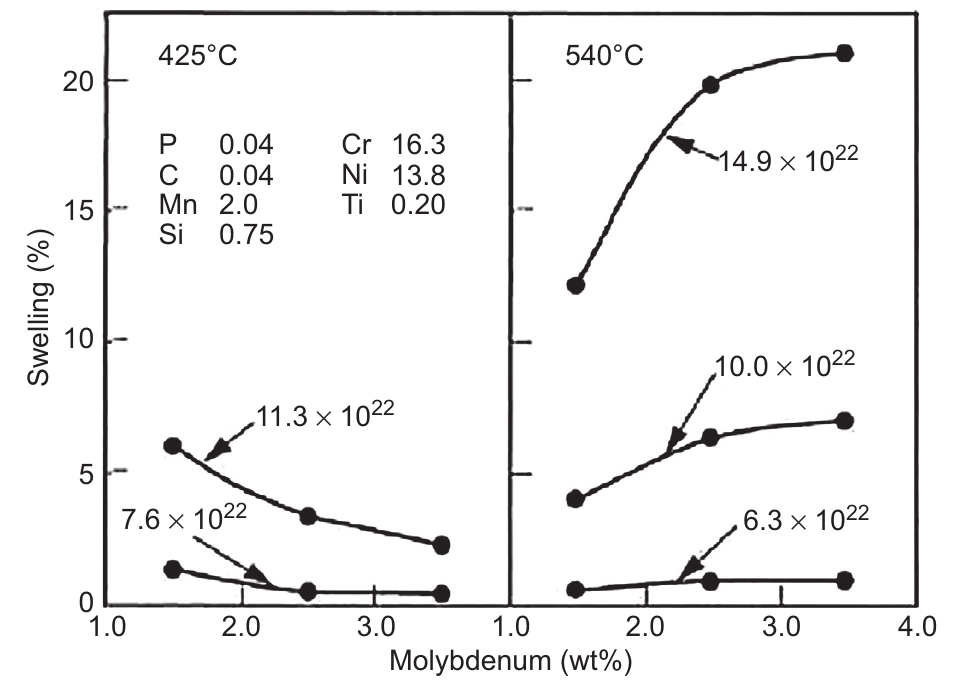
\includegraphics[width=7.0cm]{chapters/background_austenitic_steels_in_nuclear/plots/moswelling.png}
    \caption{Graph caption}
    \label{image:flux1}
  \end{center}
\end{figure}